\hypertarget{basic-settings}{%
\subsection{Basic Settings}\label{basic-settings}}

Here we present the basic setup of the model.

\hypertarget{coordinate-system}{%
\subsubsection{Coordinate System}\label{coordinate-system}}

The coordinate system of the atmospheric model consists of longitude \(\lambda\), latitude \(\varphi\), and normalized pressure \(\eta\) (definitions are given below), each of which is treated as
orthogonal. However, \(z\) is used for the vertical coordinate in the ground, which is treated in a land physics component.

Longitude is discretized at equal intervals (\texttt{SUBROUTINE:~{[}SETLO{]}} in asetc.F).

\begin{eqnarray}
\begin{aligned}
\lambda_i = 2 \pi \frac{i-1}{I},  \;\;\; i = 1, \ldots I.\end{aligned}
\end{eqnarray}

Latitude grids \(\varphi_j\) are derived from the Gauss-Legendre integral formula (\texttt{SUBROUTINE:~{[}SETLA{]}} in asetc.F). This is the zero point of the Legendre polynomial of order J with
\(\mu = \sin \varphi\) as the argument (\texttt{SUBROUTINE:~{[}GAUSS{]}} in uspst.F). If J is large, we can approximate

\begin{eqnarray}
\begin{aligned}
\varphi_j =  \pi \left( \frac{1}{2}- \frac{j-1/2}{J} \right), \;\;\; j = 1, \ldots J.\end{aligned}
\end{eqnarray} Usually, the grid spacing of longitude and latitude is taken to be approximately equal to \(J = I/2\), based on the triangular truncation of the spectral method.

Air pressure \(p\) is defined at half-integer levels (\(p_{k+1/2},\ k = 1, 2, \ldots K\)) using the following formula using constants \(A_{k+1/2},\ B_{k+1/2}\):

\begin{eqnarray}
\begin{aligned}
p_{k+1/2} = A_{k+1/2} +B_{k+1/2}\,p_s,\end{aligned}
\end{eqnarray} where \(A_{1/2}=A_{K+1/2}=0,\ B_{1/2}=1,\ B_{K+1/2}=0\) and thus \(p_{1/2}=p_s,\ p_{K+1/2}=0\). Therefore, the normalized pressure \(\sigma\equiv p/p_s\) can be written as below:

\begin{eqnarray}
\begin{aligned}
\sigma_{k+1/2} = \frac{A_{k+1/2}}{p_s} +B_{k+1/2}.\end{aligned}
\end{eqnarray}

Furthermore, a hybrid normalized pressure \(\eta\) is defined as below:

\begin{eqnarray}
\begin{aligned}
\eta_{k+1/2} = \frac{A_{k+1/2}}{p_0} +B_{k+1/2},\ \ \ p_0\equiv 1000\ \mathrm{hPa}.
\end{aligned}
\end{eqnarray}

Since \(A_{k+1/2},\ B_{k+1/2}, p_0\) are constants, \(\eta_{k+1/2}\) is also a constant and we use it as the vertical coordinate of the atmopheric model. However, as described in Chapter 2, basic
equations are descretized in such a way that \(\eta_{k+1/2}\) does not explicitly appear and \(\sigma_{k+1/2}\) is used instead to commonize source codes with the \(\sigma\)-coordinate system used in
MIROC 5.

Air pressure \(p_k\) at integer levels (\(p_k,\ k=1,2,\ldots K)\) is interpolated from half-level pressure as below:

\begin{eqnarray}
\begin{aligned}
p_k = \left\{ \frac{1}{1+\kappa}
\left( \frac{  p^{\kappa +1}_{k-1/2}
- p^{\kappa +1}_{k+1/2}      }
{ p_{k-1/2} - p_{k+1/2} }
\right)
\right\}^{1/\kappa}.
\end{aligned}
\end{eqnarray}

Full-level pressure in a 80-level configuration is shown in Fig. (\ref{levels}). While lower layers follow the terrain, upper layers are isobaric, and the two are smoothly connected.

\begin{figure}
\centering
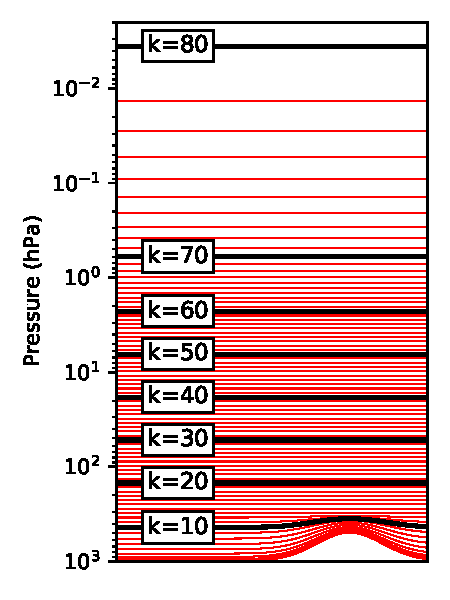
\includegraphics{../figures/levels.pdf}
\caption{Default arangement of vertical levels for 80-level simulations.}
\end{figure}

All prognostic variables are defined either on a grid of \((\lambda_i, \varphi_j, \eta_k)\) or \((\lambda_i, \varphi_j, z_l)\). (The underground level, \(z_l\), is described in the section on physical
processes.)

In the time direction, the prognostic equations are discretized at evenly spaced \(\Delta t\) and time integration is performed. However, \(\Delta t\) may change in cases where the stability of the
time integration is insufficient.

\hypertarget{physical-constants}{%
\subsubsection{Physical Constants}\label{physical-constants}}

The basic physical constants are shown below (\texttt{SUBROUTINE~{[}PCONST{]}} in apcon.F).

\begin{eqnarray}
\begin{array}{llll}
\hline \text { Element } & \text { Symbol } & \text { Unit } & \text { Value } \\
\hline \text { Earth radius } & a & \mathrm{~m} & 6.37 \times 10^{6} \\
\text { Gravitational acceleration } & g & \mathrm{~m} \mathrm{~s}^{-2} & 9.8 \\
\text { Atmospheric specific heat at constant pressure } & C_{p} & \mathrm{~J} \mathrm{~kg}^{-1} \mathrm{~K}^{-1} & 1004.6 \\
\text { Atmospheric gas constant } & R & \mathrm{~J} \mathrm{~kg}^{-1} \mathrm{~K}^{-1} & 287.04 \\
\text { Latent heat of water evaporation } & L & \mathrm{~J} \mathrm{~kg}^{-1} & 2.5 \times 10^{6} \\
\text { Water vapor specific heat at constant pressure } & C_{v} & \mathrm{~J} \mathrm{~kg}^{-1} \mathrm{~K}^{-1} & 1810 \\
\text { Gas constant of water } & R_{v} & \mathrm{~J} \mathrm{~kg}^{-1} \mathrm{~K}^{-1} & 461 \\
\text { Density of liquid water } & d_{H_{2} O} & \mathrm{~kg} \mathrm{~m}^{-3} & 1000 \\
\text { Saturated vapor pressure at } 0{ }^{\circ} \mathrm{C} & e^{*}(273 \mathrm{~K}) & \mathrm{Pa} & 611 \\
\text { Stefan-Bolzman constant } & \sigma_{S B} & \mathrm{~W} \mathrm{~m}^{-2} \mathrm{~K}^{-4} & 5.67 \times 10^{-8} \\
\text { Kárman constant } & k & & 0.4 \\
\text { Latent heat of ice melting } & L_{M} & \mathrm{~J} \mathrm{~kg}^{-1} & 3.4 \times 10^{5} \\
\text { Freezing point of water } & T_{M} & \mathrm{~K} & 273.15 \\
\text { Constant pressure specific heat of water } & C_{w} & \mathrm{~J} \mathrm{~kg}^{-1} & 4200 \\
\text { Freezing point of seawater } & T_{I} & \mathrm{~K} & 271.35 \\
\text { Specific heat ratio of ice at constant pressure } & C_{I}=C_{w}-L_{M} / T_{M} & & 2397 \\
\text { Water vapor molecular weight ratio } & \epsilon=R / R_{v} & & 0.622 \\
\text { Coefficient of virtual temperature } & \epsilon_{v}=\epsilon^{-1}-1 & & 0.606 \\
\text { Ratio of specific heat to gas constant } & \kappa=R / C_{p} & & 0.286 \\
\hline
\end{array}
\end{eqnarray}
